% Chapter 5 from the standard thesis template
%   with a full page figure and a sideways table.

%Chapter 5 discusses the Experimental setup and experiments used and how I evaluated the performance of the radiometer.

\chapter{EVALUATION SETUP AND EXPERIMENTAL DESIGN}\label{ch:exp_design}
The experiments outlined in this chapter are used to demonstrate and verify that a software defined radio (SDR) base radiometer can perform on par with a traditional radiometer.  In addition, these experiments are designed to demonstrate that a SDR based radiometer can provide functionality not typically found in traditional radiometers. 

Four experiments are described.  Experiment one verifies our SDR-based radiometer by comparing its operation to a square-law detector, a device typically used within a traditional radiometer.  Experiment two evaluates the sensitivity and stability of our SDR-based radiometer.  Experiment three evaluates our SDR-based radiometer's ability to mitigate an interfering signal in comparison to the behavior of a traditional radiometer in the presence of an interfering signal.  Experiment four's purpose is to further examine the impact of our frequency notching approach for Radio Frequency Interference (RFI) mitigation on radiometer sensitivity.

\section{Experiment I - Software Defined Radiometer Verification and Calibration}\label{Exp1}
%Experiment 1
%Why is this experiment being run?
%What type of data will you collect?
%What is the experimental setup?

This experiment is designed to verify our SDR-based radiometer functions as expected.  Its behavior is compared against an analog square-law detector, which is commonly used in traditional radiometers.  

\ \\

To verify the results of the information that the software defined radio is obtaining a square-law detector is used to measure the power of the incoming signal in parallel to the SDR-based radiometer.  This signal is split using a power divider so that the information will be the same to both devices.  This power divider ideally would divide the signal so that the resulting signal is 3 dB lower, plus the insertion loss, and is equal between both ports.  The splitter used in this thesis was tested and verified that it does split the signal with a slight difference between port one and port two.  This difference was measured to be .1 dB which is well within the .3 dB specified for this power splitter.  This allows us to verify the software defined radio with a proven system.  

\subsection{Experimental setup} \label{exp1_setup}

Figure \ref{Exp1_Block} shows a block diagram of the experimental setup.  A matched load is used to simulate our source signal.  This matched load is then submerged in temperature baths.  These baths use Liquid Nitrogen (LN2), which is known to boil at 77 Kelvin, and an ice water bath which is known to be at 273.15 Kelvin.  The temperature of these baths were monitored with a thermometer that had an accuracy of $\pm 1$ degree Celsius.  The load was submersed in each bath for a minimum of 2 minutes to allow it to reach the same temperature as the bath.  The physical temperature of this matched load is then the noise temperature the radiometer sees and can be used to calibrate the radiometer.  

{\begin{figure}[h!tb] \centering
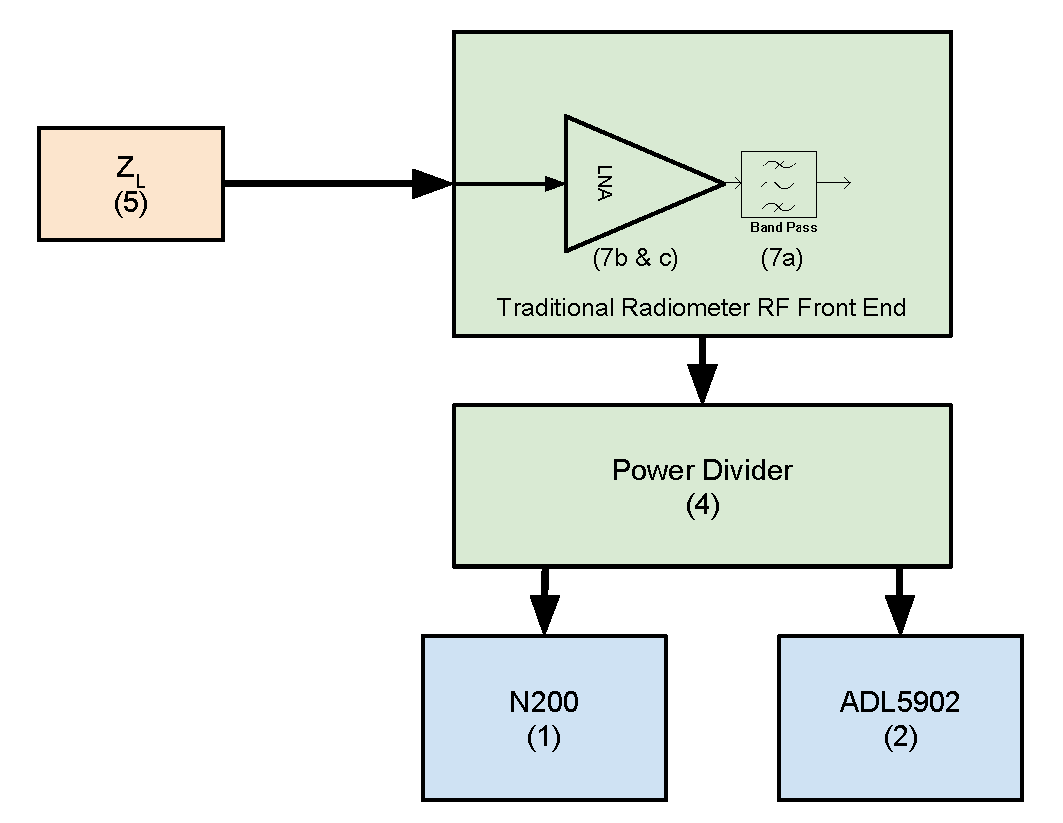
\includegraphics[width=13cm]{Images/Exp_1_Setup.pdf}
\isucaption{Block diagram of Experiment 1 setup.}
\label{Exp1_Block}
\end{figure}
}

The radiometer RF front end provides the amplification needed for our experiments.  Figure \ref{ISURF} shows an image of the RF front end, with the LNAs and band-pass filters marked.  After the signal has been amplified, we divide the signal between the square-law detector (ADL5902) and the software defined radio (N200).  The N200 is then connected to a personal computer running XUbuntu Linux and GNURadio.

{\begin{figure}[h!tb] \centering
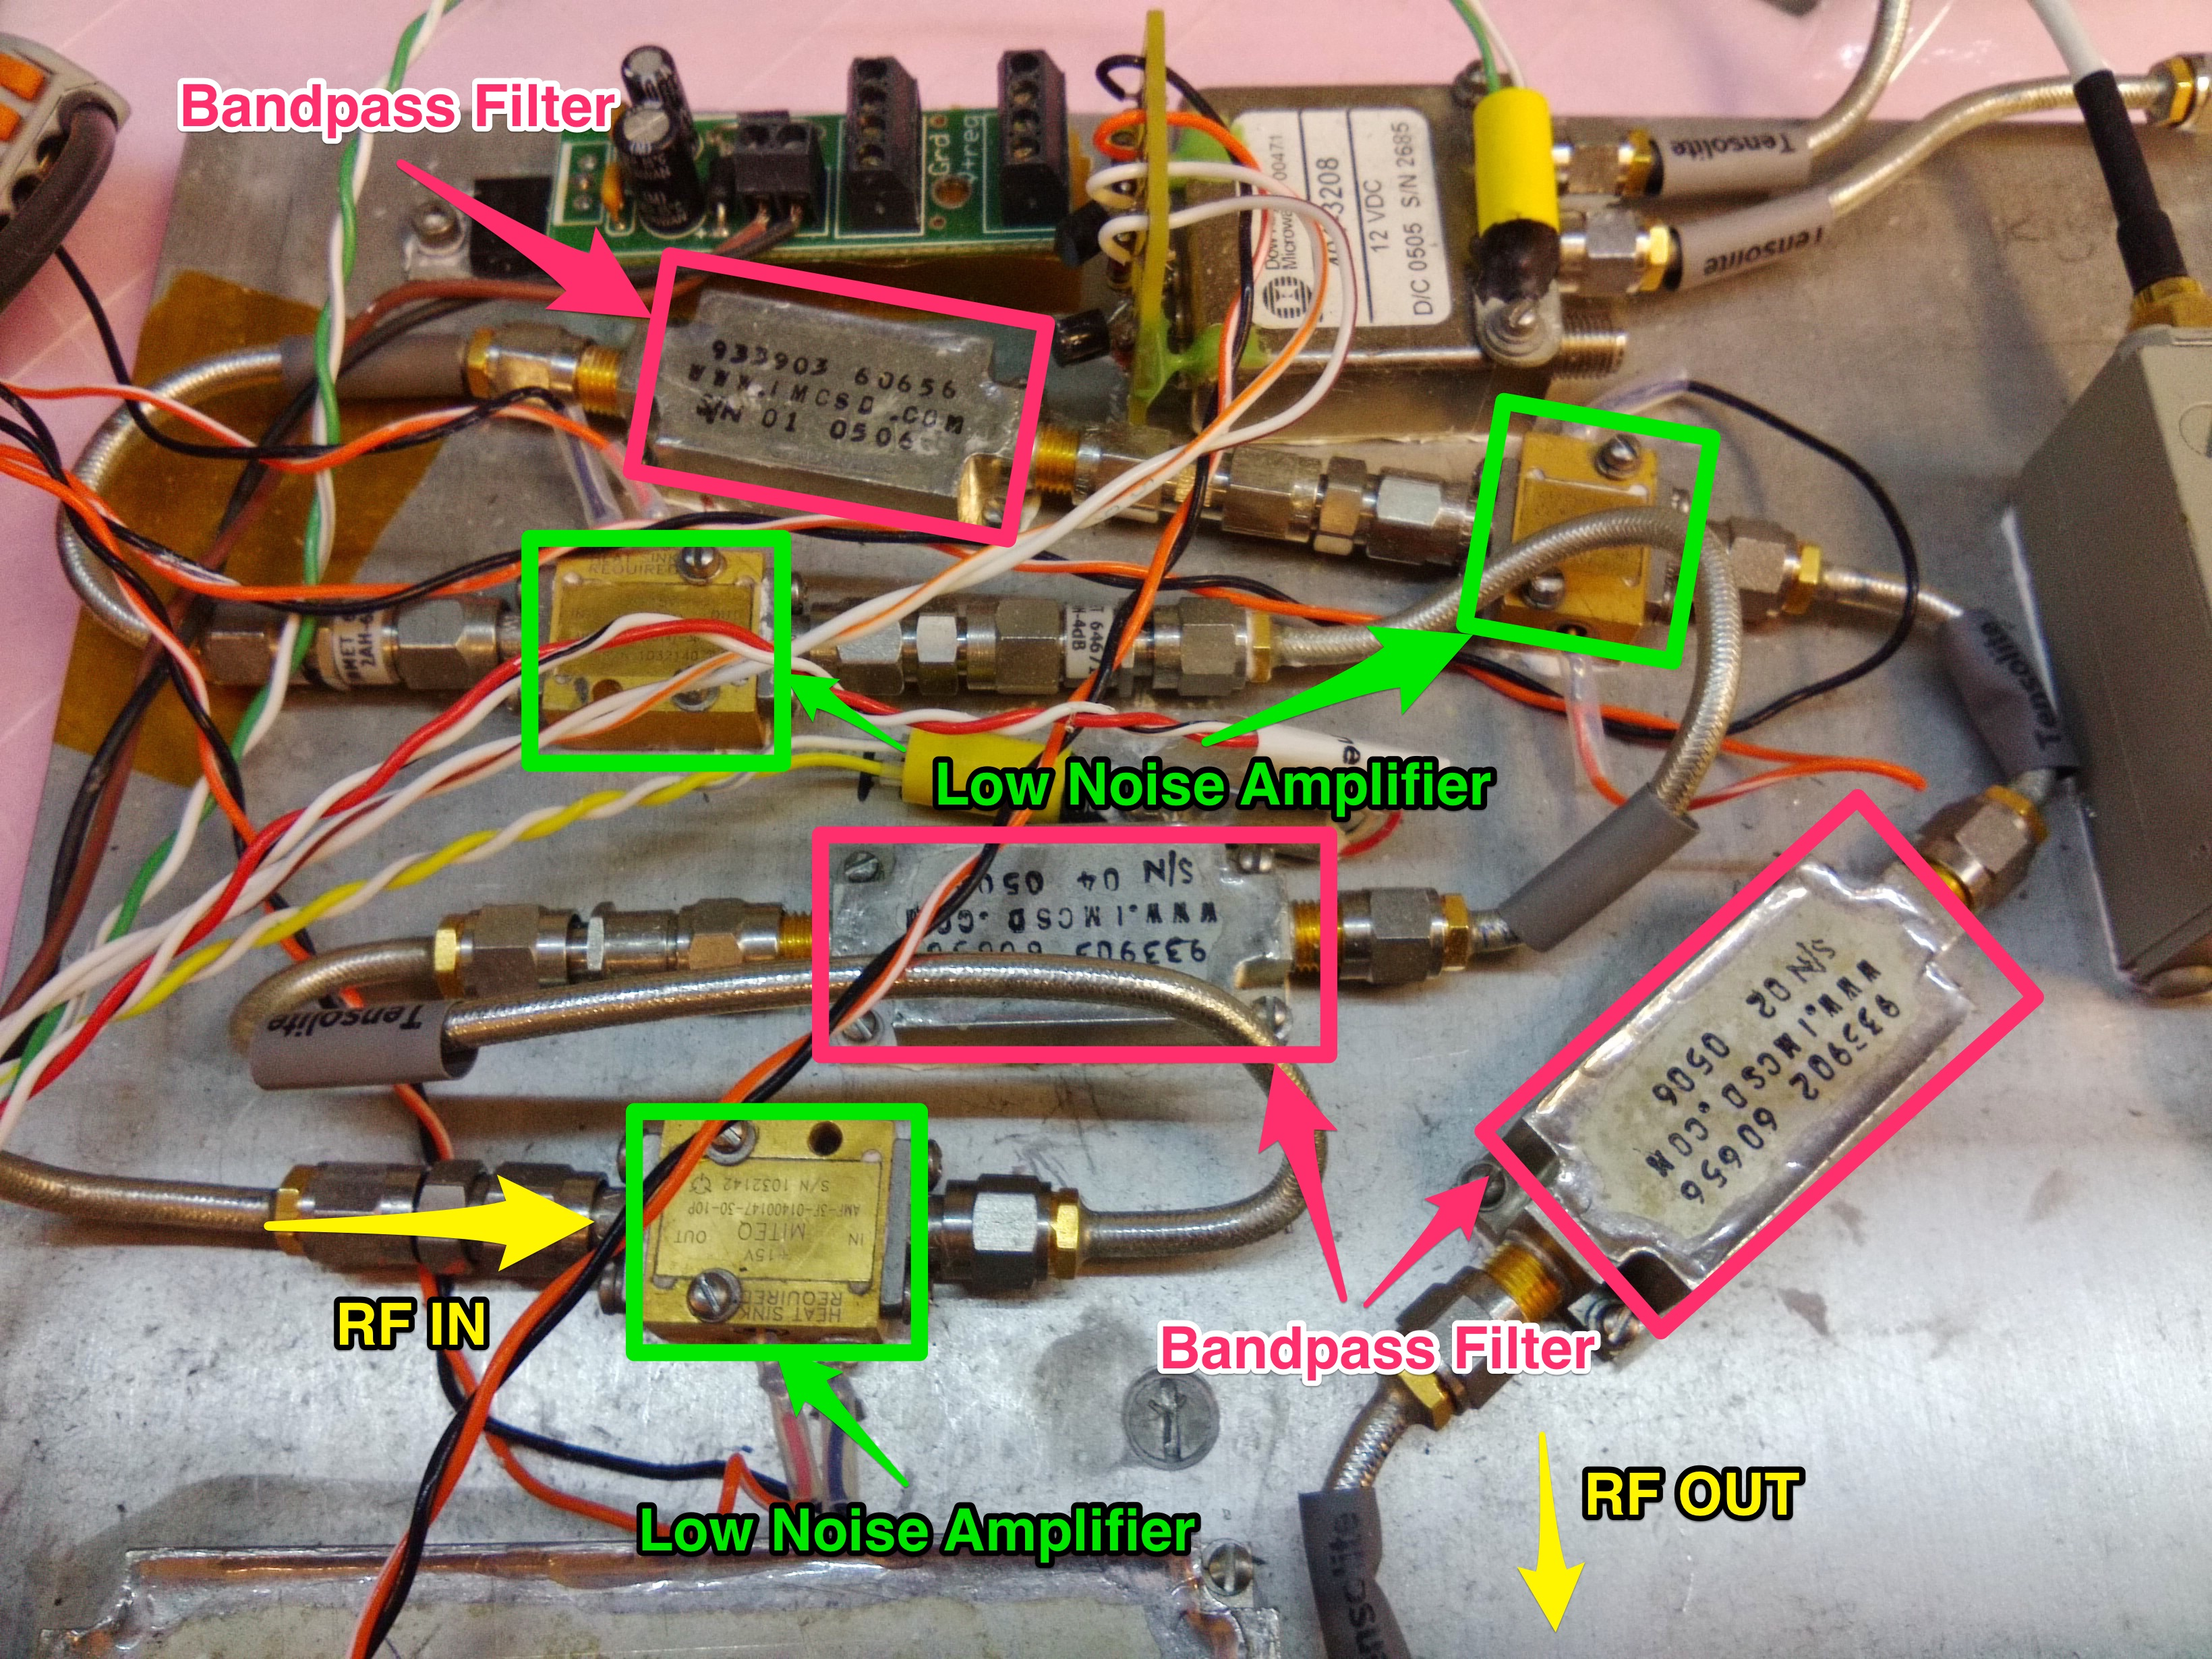
\includegraphics[width=\textwidth]{Images/ISU_RF_noted.jpg}
\isucaption{The radiometer RF front end, with LNAs and band-pass filters used in the experiments.}
\label{ISURF}
\end{figure}
}

The following hardware was used and has also been marked on Figure \ref{Exp1_Block}:

\begin{enumerate}
\item N200 Software Defined Radio with DBSRX2 Daughter-board
\item ADL5902 Square-law detector
\item National Instruments USB-6009 Data Acquisition Unit (not shown in Figure \ref{Exp1_Block})
\item ZN2PD-20-S+ Power Divider
\item 50-ohm matched load ($Z_L$)
\item Rigol DP832 Power Supply (not shown in Figure \ref{Exp1_Block})
\item Radiometer RF Front End
\begin{enumerate}
\item 4 x Integrated Microwave Bandpass filters (1400 - 1425 MHz)
\item 2 x Miteq AMF-3F-01400147-30-10P LNA
\item 1 x Miteq AMF-2F-01400147-04-10P LNA
\end{enumerate}
\end{enumerate}

\subsection{Data collection}\label{exp1_data}

Two sets of data are produced with this experiment.  First, data is generated from the software defined radio using GNURadio.  Second, data is generated from a data acquisition device (USB-6009) that is attached to the square-law detector.  Data from each is stored to a local computer running the appropriate software.

\emph{Software Defined Radio Data.}  The software defined radio based radiometer is configured with a bandwidth of 10 MHz and an integration time of two seconds.  It is centered on a frequency of 1.406 GHz which allows it to operate within the mechanical band-pass filters.

The data from the software defined radio is stored in files generated from GNURadio.  GNURadio uses a sink block to output the data to either a screen, socket connection such as TCP/IP, or a file.  As shown in Figure \ref{filesink}, a file sink block is used to output the data to a file.  The flow of data to this sink is controlled by a valve block.  This allows the user to turn on and off recording of the data.

{\begin{figure}[h!tb] \centering
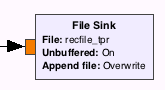
\includegraphics[width=5cm]{Images/TPR_Filesink.png}
\isucaption{The File Sink block used in GNURadio.  Source:  GNURadio}
\label{filesink}
\end{figure}
}

There are two types of files the SDR generates.  The first type of file is the I (in-phase) and Q (quadrature phase) data points.  This file is stored in little-indian format as complex values.  Due to the sampling rate, it is not uncommon for this file to grow quite large, usually several gigabytes of data for a 10-15 minute run.  However, this file can then be fed back through GNURadio later to be played back if needed, and it contains the information needed to completely recreate the signal.

The second file type is the total power values generated from the total power block in GNURadio.  A diagram of this block can be found in Appendix \ref{appendix1} (Figure \ref{TPR_GRC}), and its source code can be found in Appendix \ref{appendix1}.  This file also uses a little-endian format, however this file only has real values.  This file is also much smaller than the file that contains the I and Q data points due to decimation of the data.  A typical file size is 50 - 100 kB for a 10 to 15 minute run.  

\emph{Square-law detector data.}  The square-law detector used (ADL5902) outputs total power information as an analog voltage that is linearly proportional to the RF power measured.  The Analog Devices ADL5902 is a single Integrated Circuit (IC) that contains a square-law detector and necessary amplification for the output signal and is shown in Figure \ref{square_law} .  This device operates from 50 MHz to 9 GHz and can detect power as low as -60 dBm.  The output voltage from the square-law is amplified to a range from zero to five volts with a calibrated output of 53.7 mV/dB.  

Testing was done on the square-law detector to verify linearity and proper operation of the square-law detector.  This test involved sending a known signal into the square-law detector and changing the amplitude at set intervals.  This was then graphed and is shown in Figure \ref{square_law_linear}.  This graph shows that as we changed the input power in linearly, the output measured from the square law detector also changed linearly.

{\begin{figure}[h!tb] \centering
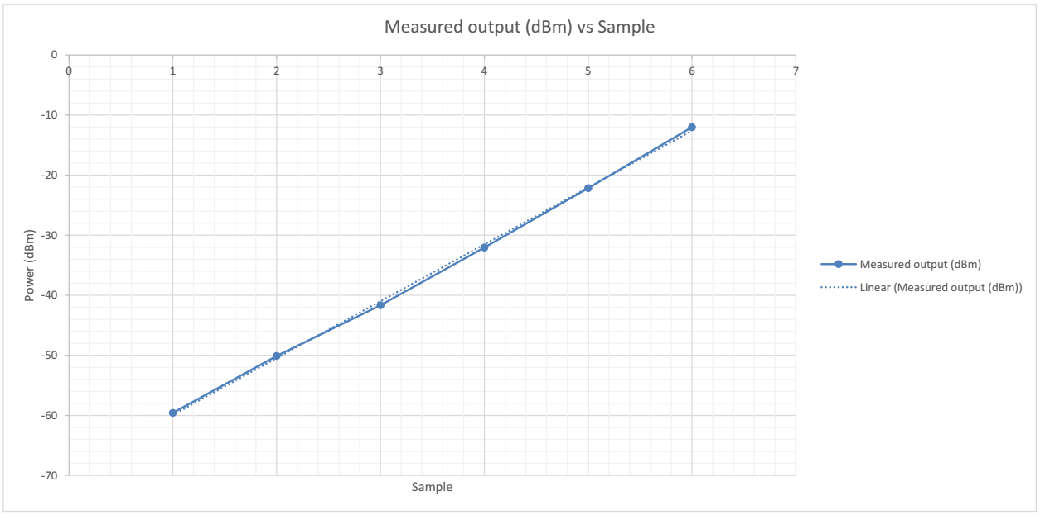
\includegraphics[width=\textwidth]{Images/square_law_linear1.pdf}
\isucaption{A graph of the power output of the square law detector.}
\label{square_law_linear}
\end{figure}
}

To capture the voltage output from the ADL5902, a data acquisition unit (DAQ) is used.  The National Instruments USB-6009 DAQ unit was selected as it met the requirements for an easy to use yet high enough resolution to obtain accurate information.  The USB-6009 unit has 8 analog inputs that can sample at 48 KSPS with a resolution of 14-bits.  

To use the USB-6009, a fairly simple Lab View program was created to obtain, display and store the data from the ADL5902.  This program retrieved information from the USB-6009 and stored the data in both Labview's binary format and in a more human friendly ASCII format.  A GUI program, shown in Figure \ref{labviewgui}, is used to control and display the data.  This made obtaining the data and using the device straightforward.

{\begin{figure}[h!tb] \centering
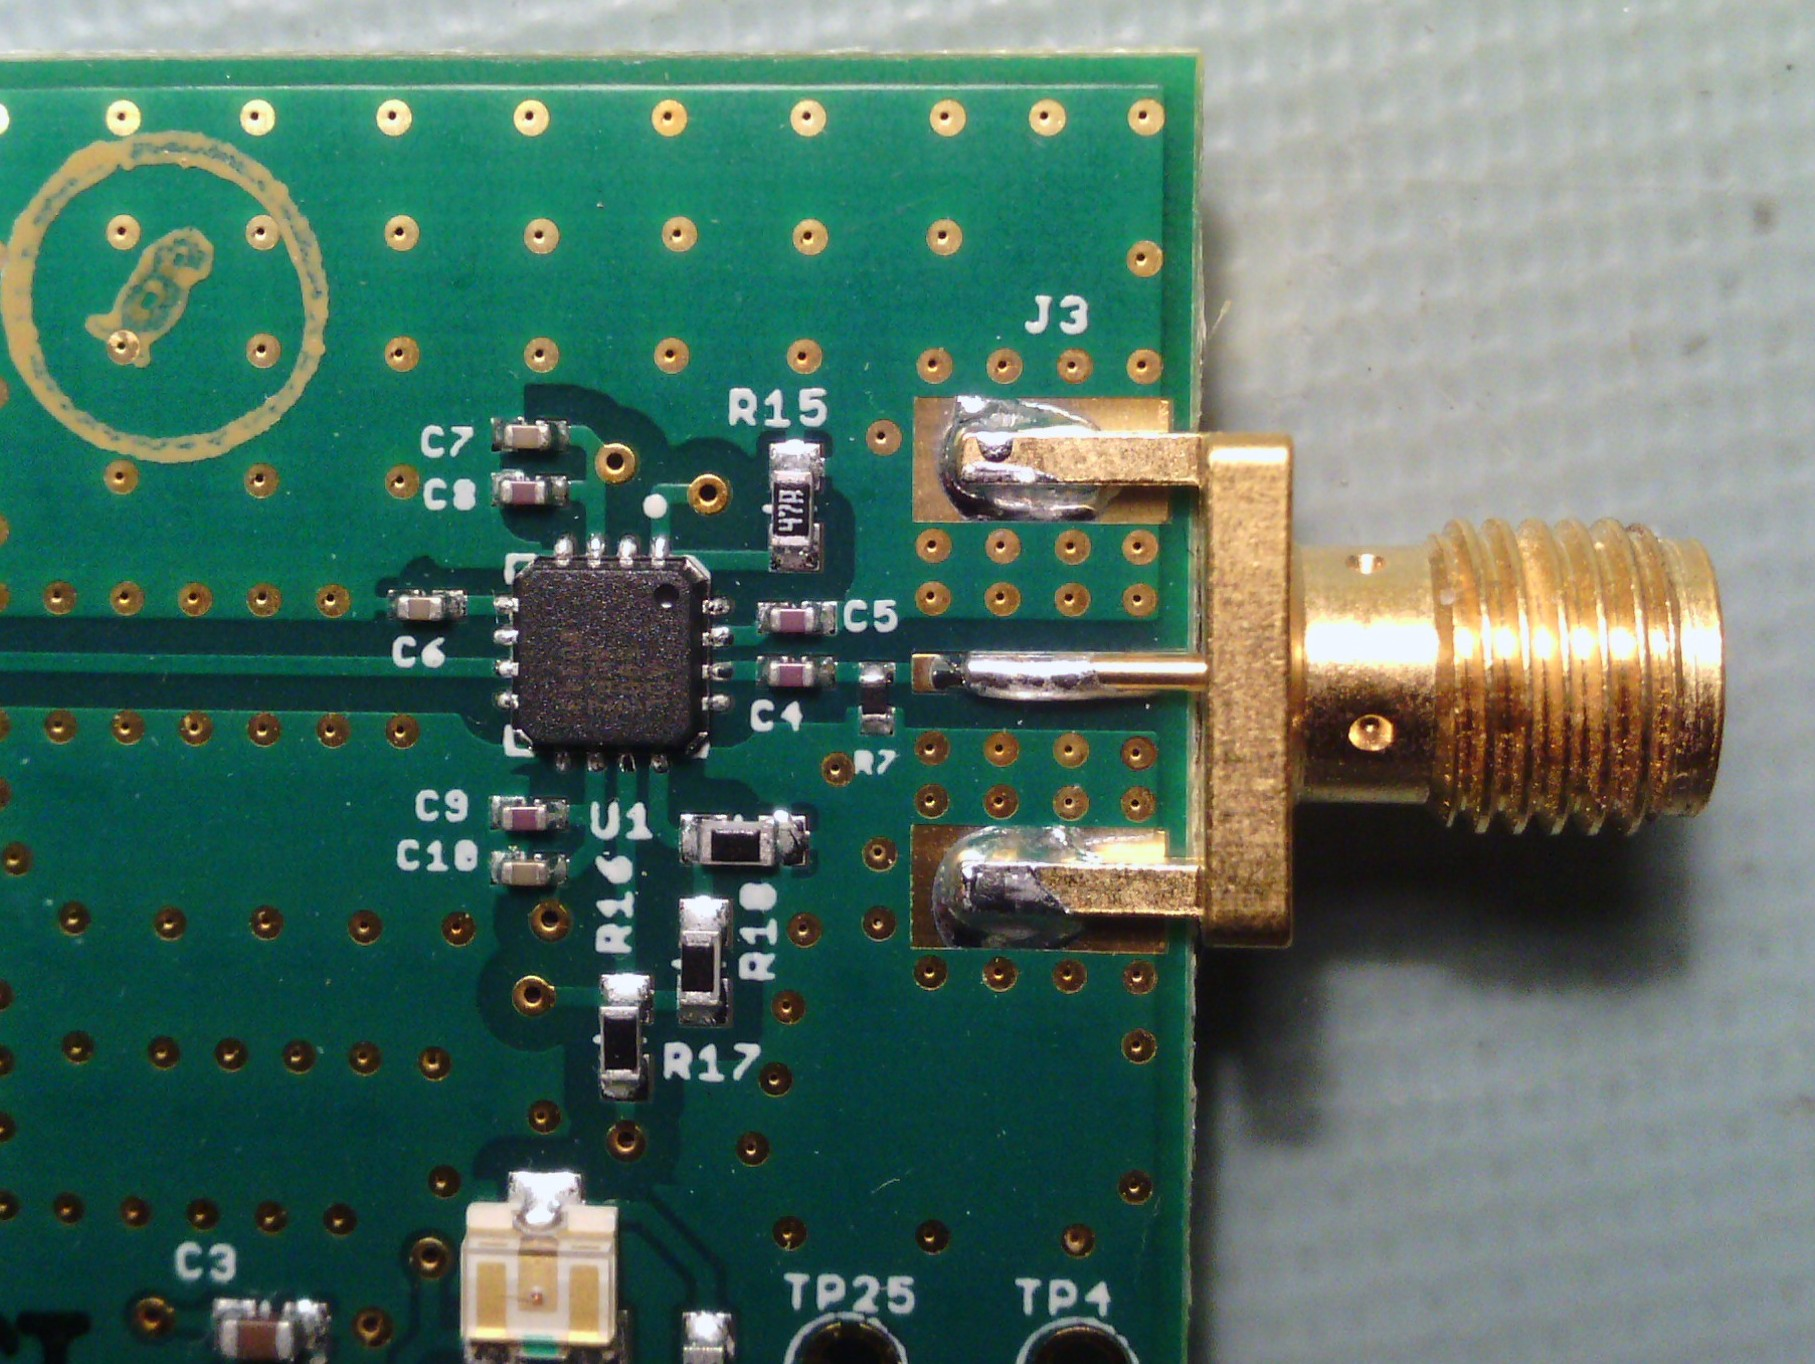
\includegraphics[width=7cm]{Images/adl5902.jpg}
\isucaption{The ADL50902 IC on a demonstration board.}
\label{square_law}
\end{figure}
}

{\begin{figure}[h!tb] \centering
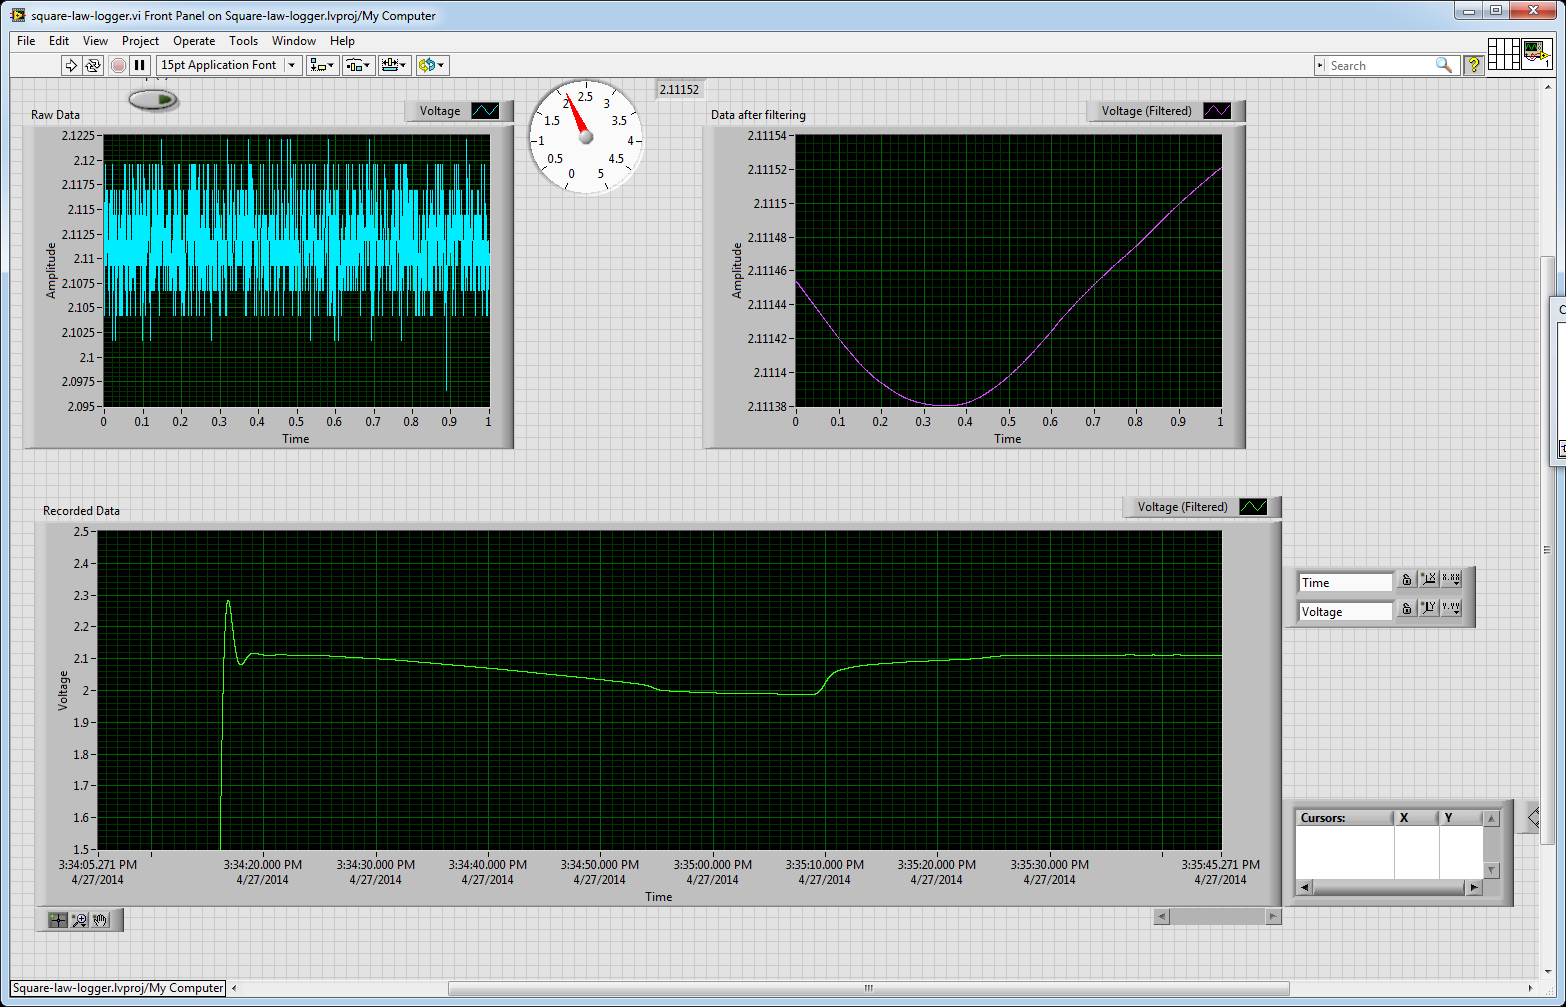
\includegraphics[width=\textwidth]{Images/labviewGUI.png}
\isucaption{A screenshot of the Labview GUI interface.}
\label{labviewgui}
\end{figure}
}

For rapid development, the National Instruments DAQ assistant was used to quickly configure and setup the USB-6009.  Labview also includes blocks that allows us to easily record the data to a file and to use a low pass filter.  The filter used is then configured to have a cutoff frequency that is equivalent to an integration time of 2 seconds to match the software defined radio.  These blocks made up most of the program and resulted in a program that was quickly made.  Figure \ref{labviewblock} shows the blocks used and the wiring of the blocks.

{\begin{figure}[h!tb] \centering
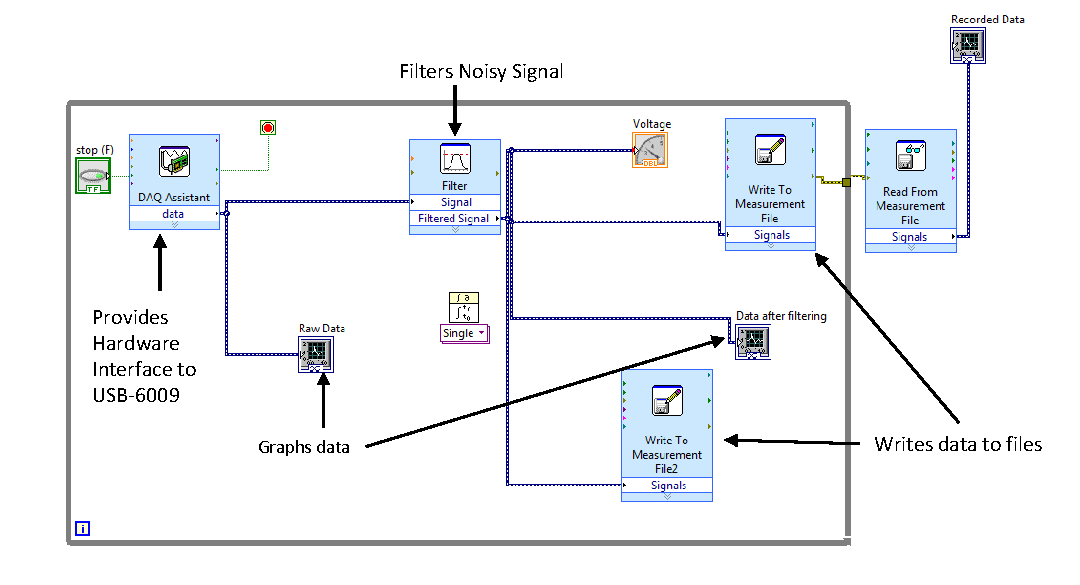
\includegraphics[width=\textwidth]{Images/labview_diagram.pdf}
\isucaption{A screenshot of the Labview block diagram.}
\label{labviewblock}
\end{figure}
}

\section{Experiment II - Sensitivity and Stability Evaluation}\label{Exp2}

In this experiment, we evaluate the sensitivity and stability of a SDR-based radiometer.  This is evaluated both experimentally and statically.  

\subsection{Experimental setup} \label{exp2_setup}
The experimental setup used for experiment two is the same as outlined in section \ref{exp1_setup}.  A longer soak time is used to verify the stability of the radiometer.

\subsection{Data collection}
The data collected for this experiment were the total power measurements made from the SDR-based radiometer.  These measurements uses the same method as outlined in section \ref{exp1_data}.  A longer soak time was used for this experiment where the matched load was in LN2 for approximately five hours before the LN2 boiled out.  

\section{Experiment III - Interfering Signal Mitigation}\label{Exp3}

In this experiment, we generate an interfering signal and then mitigate the signal using a software defined filter.  A square-law detector is hooked up in parallel to measure the same signal, but is not provided with a mitigation mechanism.  We then compare the two signals to verify that the SDR-based radiometer can mitigate the interfering signal, while continuing to make useful total power measurements.

This experiment was designed to determine whether or not a SDR-based radiometer can cope with an interfering signal.  This test injects a known signal at 1.406 GHz to interfere with the normal operation of the radiometer.  The amplitude of this signal is then incremented and decremented at various times during the test.  This was done to reflect a possible real world scenario and to make it easy to identify the interfering signal with the square-law detector, which only measures power.  

In order to mitigate the offending signal, a filter was designed to remove the offending signal.  The design of the filter used a program that is part of the GNURadio software package, called the GNU Radio Filter Design tool.  Figure \ref{GRC_Filter_DSN} shows a screen shot of this tool when designing the band-reject filter for this application.  

This tool generates filter values (also called taps) that GNURadio will use for defining the filter.  The GUI program, shown in Figure \ref{GRC_Filter_DSN}, allows us to interactively create a filter.  Because this tool is part of the GNURadio package, it also includes a command line interface to the program.  This allows us to call the program from within GNURadio to integrate this functionality into our SDR-based radiometer.  

\begin{figure}[h!tb] \centering
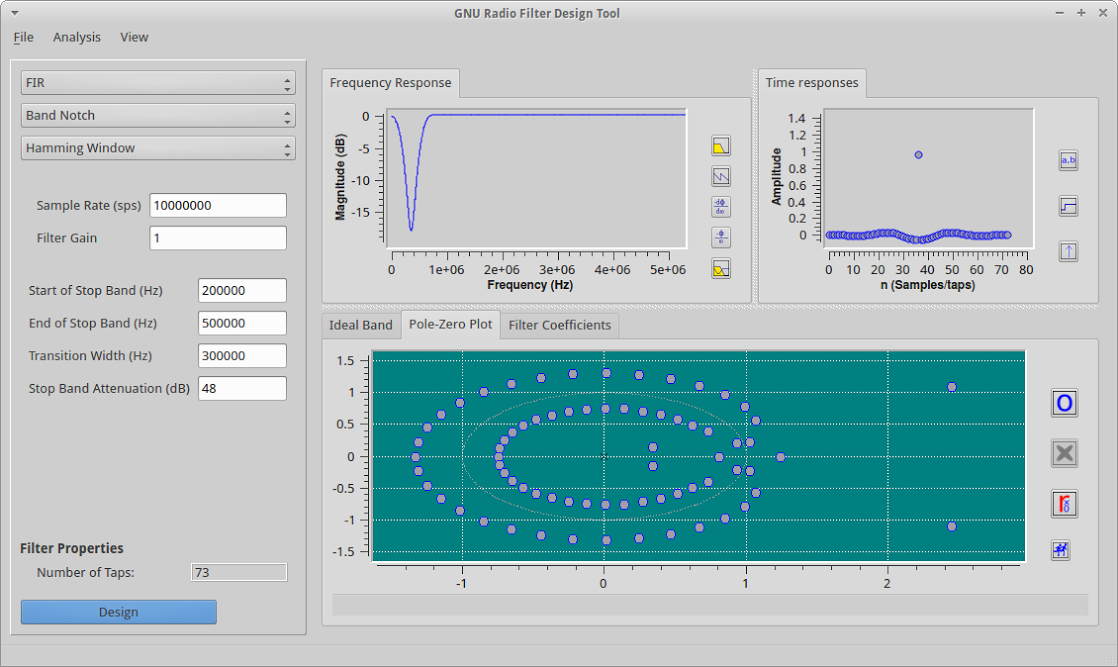
\includegraphics[width=\textwidth]{Images/GNURadio_Filter_dsn.png}
\isucaption{Image of the GNU Radio Filter Design tool}
\label{GRC_Filter_DSN}
\end{figure}  

\subsection{Experimental setup} \label{exp3_setup}

The setup for this experiment is similar to the setup outline in section \ref{Exp1}.  In addition, a second software defined radio was added to inject an offending signal into the RF signal chain.  This software defined radio was configured to operate as a signal generator to create the offending signal.  

Our signal generator is the HackRF One (or just HackRF), shown in Figure \ref{HackRF}.  This SDR is cheaper, and has lower specifications than the Ettus Research N200 used as the SDR-based radiometer.  However, it allows for transmission of a signal and it suits our needs for the purpose of a signal generator.  The signal the HackRF generates is a sinusoidal signal centered at 1.406 GHz.  The amplitude of this sinusoidal signal is then adjusted accordingly. 

As stated, the quality of this SDR is lower than the Ettus Research N200 SDR.  As such the output signal is not as clean as one might expect.  This can be seen in Figure \ref{spectrum_filter} where two smaller signals are present.  These are harmonics generated due to the Local Oscillator (LO) and the Intermediate Frequency (IF) used in the setup.  However, this did not present an issue as the filter was designed to filter the main signal at 1.406 GHz and the two smaller harmonic peaks.

\begin{figure}[h!tb] \centering

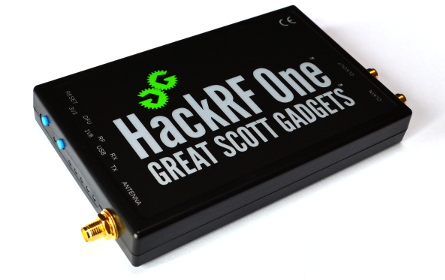
\includegraphics[width=12cm]{Images/hackrf.jpg}
\isucaption{Image of the HackRF used to generate the offending signal. (Image from Great Scott Gadgets - www.greatscottgadgets.com)}
\label{HackRF}
\end{figure} 

The HackRF generates a sinusoidal wave at a fixed frequency of 1.406 GHz and can be seen in Figure \ref{spectrum_interfering}.  In this experiment, the signal amplitude is changed at different times during the experiment.  Because the signal from this device is relatively large, 26 dB of attenuation is inserted between the HackRF and the first LNA to avoid over-powering the LNAs.  

The amplitude is controlled from a program called \emph{osmocom\_siggen}.  Osmocom was originally developed to communicate with OsmocomSDR hardware.  However, it has been expanded to include the HackRF and Ettus Research hardware.  The \emph{osmocom\_siggen} program provides a GUI to set the frequency, amplitude and type of the signal generated.  

\subsection{Data collection}

The data collected for this experiment includes both the total power measurements from the SDR-based radiometer and the square-law data.  Section \ref{exp1_data} explains in detail the setup and configuration of the equipment used to collect this data.

\section{Experiment IV - Performance Impact of Interfering Signal Mitigation}\label{Exp4}

In this experiment we examine the impact of filtering an interfering signal on the sensitivity of the SDR-based radiometer and how reducing our overall bandwidth affects the total power received by the radiometer.

\subsection{Experimental setup} \label{exp4_setup}

In this experiment, we set up our experiment as outlined in Section \ref{Exp3}.

\subsection{Data collection}

The data collected for this experiment is the total power reading measurements obtained from the software defined radio.  The data collection method is identical to the method used in Section \ref{exp1_data}.

%----------------------------------------------------------
% End of Chapter 5.  Anything below this is extra information
